\documentclass[a4paper,10pt]{article}
\usepackage[a4paper, total={167mm, 245mm}]{geometry}

\usepackage[colorlinks,linkcolor=blue,bookmarks,bookmarksopen,pdfauthor=krom]{hyperref}

\usepackage{fontspec}
\setmainfont[BoldFont={fonts/epkgobld.ttf}]{epkaisho.ttf}

\graphicspath{{images/}}

\usepackage[normalem]{ulem}
\renewcommand{\ULthickness}{0.08em}

\usepackage[compact]{titlesec}
\titlespacing{\section}{0em}{*0}{*0}
\titleformat{\section}{\normalfont\huge}{\thesection}{0em}{}

\setlength\parindent{1em}
\setlength\parskip{0em}
\renewcommand{\baselinestretch}{1.4}

\usepackage{fancyhdr}
\pagestyle{fancy}
\fancyhf{}
\renewcommand\headrulewidth{0pt}

\usepackage{tikz}
\tikzset{>=stealth} % Define Standard Arrow Tip
\definecolor{fontgreen}{RGB}{86, 158, 56}
\definecolor{fontpink}{RGB}{255, 128, 128}
\definecolor{fontyellow}{RGB}{255, 255, 128}
\definecolor{arrowblue}{RGB}{0, 146, 255}

\begin{document}

\fancyfoot[R]{\thepage}

\begin{flushright}
2016/3/26 版
\end{flushright}

\vspace{17.5em}

\LARGE
\textbf{\hskip 5em \,OpenToonz}\par
\textbf{\hskip 5em スタートアップマニュアル}\par
\textbf{\hskip 5em 導入編}

\noindent\begin{picture}(0,0)
\put(0,24){
\includegraphics[width=5em]{OpenToonzLogo}}
\end{picture}

\newpage

\phantomsection
\section*{\uline{\hskip -3em \hskip 3em □インストール手順\hskip 9em}}
\addcontentsline{toc}{section}{□ インストール手順}

\large

\noindent ① インストーラを起動します

\noindent \begin{picture}(0,0)
\put(72,-90){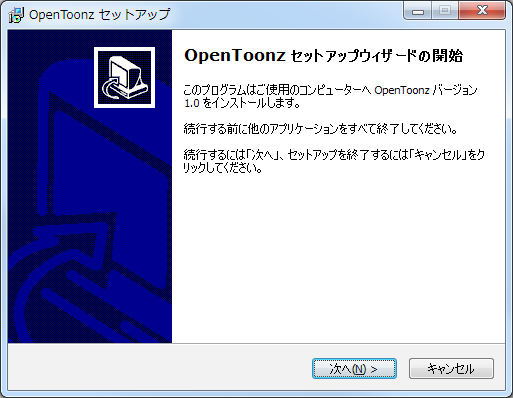
\includegraphics[width=11.5em]{InstallationProcedure1A}}
\put(257,-90){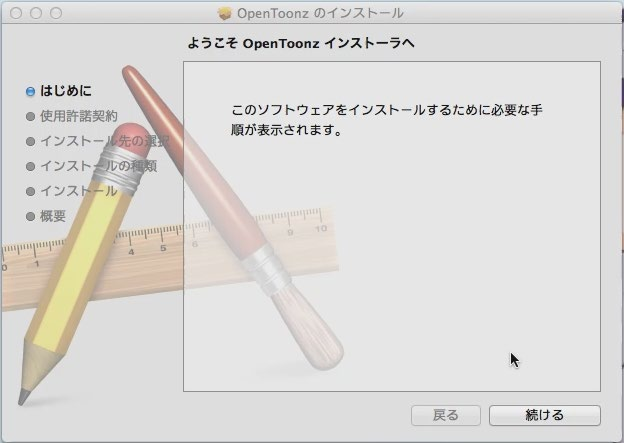
\includegraphics[width=12.5em]{InstallationProcedure1B}}
\end{picture}\\[5.5em]

\noindent ② 利用規約をよくお読みになり、同意する場合は「同意する」を押して次に進みます。

\noindent \begin{picture}(0,0)
\put(72,-90){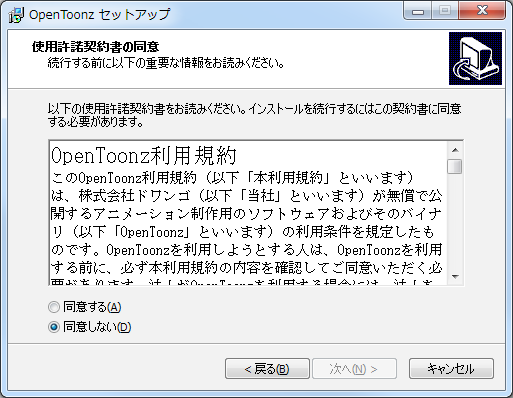
\includegraphics[width=11.5em]{InstallationProcedure2A}}
\put(257,-90){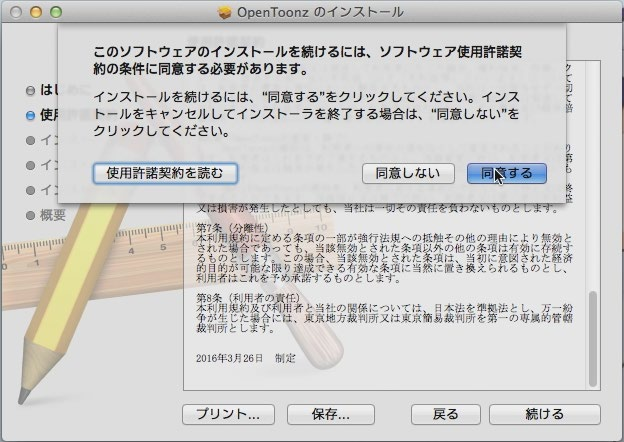
\includegraphics[width=12.5em]{InstallationProcedure2B}}
\end{picture}\\[5.5em]

\noindent ③ OpenToonz ソフトウェアのインストール先を指定します

\noindent \begin{picture}(0,0)
\put(72,-90){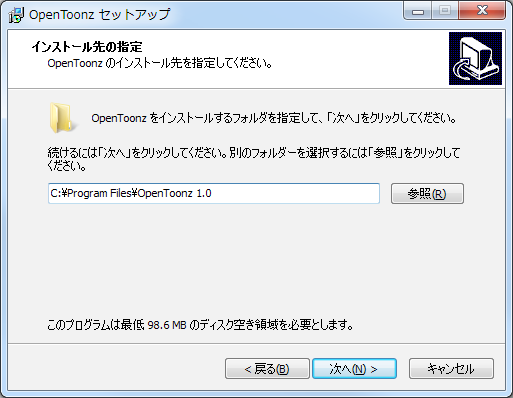
\includegraphics[width=11.5em]{InstallationProcedure3A}}
\put(257,-90){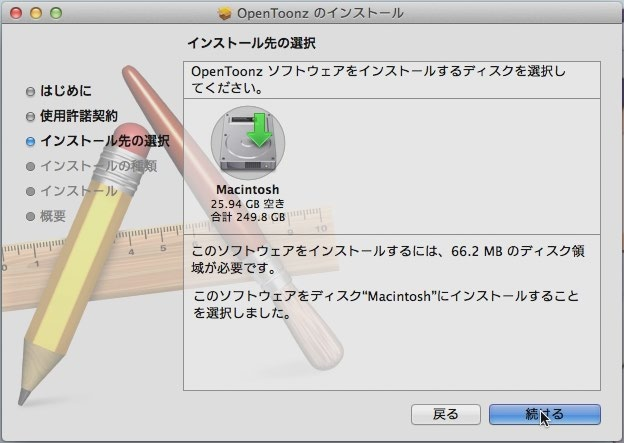
\includegraphics[width=12.5em]{InstallationProcedure3B}}
\end{picture}\\[7.5em]

\noindent ④ (Windows のみ) Stuff フォルダの保存先を指定します。\\[0.5em]
\normalsize
OS Xの場合はあらかじめ決まった場所にStuffフォルダが展開されます。\\
どちらの場合も、後で記述する方法でフォルダの位置を変更できます。\\
Windows の場合はさらに、スタートメニューとデスクトップアイコン\\
の指定を行います。

\large

\noindent \begin{picture}(0,0)
\put(329,-20){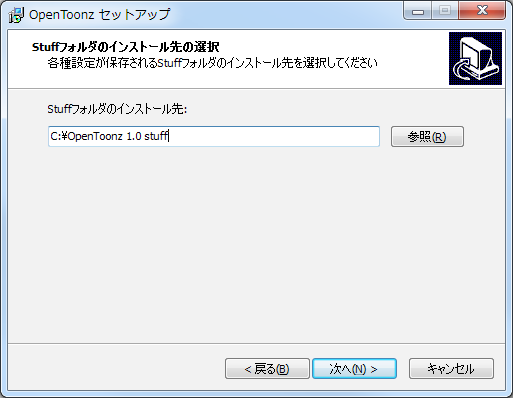
\includegraphics[width=11.5em]{InstallationProcedure4}}
\end{picture}\\[-0.5em]

\noindent ⑤ ファイルがコピーされ、インストールが完了します。

\noindent \begin{picture}(0,0)
\put(72,-98){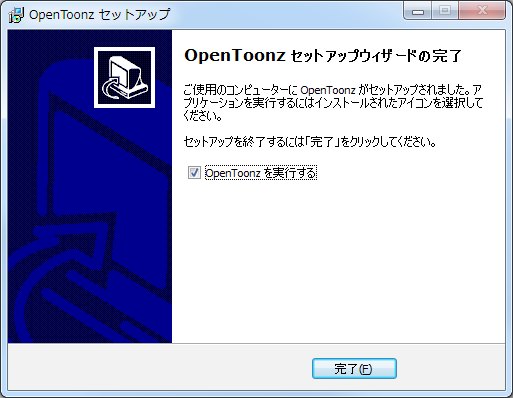
\includegraphics[width=11.5em]{InstallationProcedure5A}}
\put(257,-98){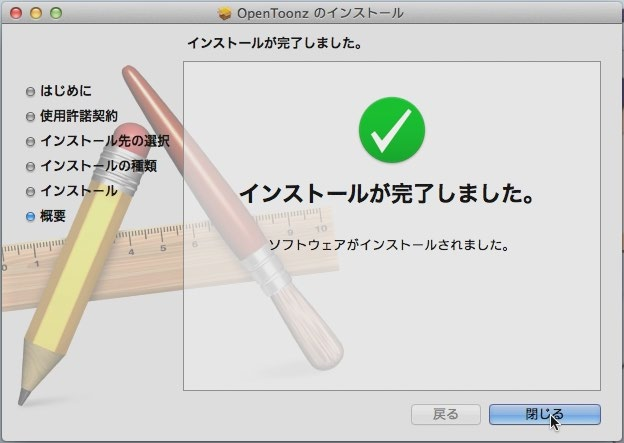
\includegraphics[width=12.5em]{InstallationProcedure5B}}
\end{picture}

\fancyfoot[R]{\thepage
\begin{picture}(0,0)
\put(-523,-50){
\includegraphics[width=58em]{OpenToonzFooter}}
\end{picture}
}

\newpage

\phantomsection
\section*{\uline{\hskip -3em \hskip 3em □ Stuffフォルダについて\hskip 6em}}
\addcontentsline{toc}{section}{□ Stuff フォルダについて}

\normalsize
\noindent Stuffフォルダは、OpenToonzの各種設定が収められたフォルダです。複数のユーザが1つの作品を制作す\\
る場合、共有しているデータフォルダ内に Stuff フォルダを作成することで、プロジェクト設定や作品共通\\
の色見本データなどを一本化することができます。\\
Stuffフォルダ内には、さらに下記の通りいくつかのフォルダがあります:\\
- cache: 画像のキャッシュデータが一時的に保管されます\\
- config: スタイルシート、翻訳ファイル等の各種設定ファイルが入っています\\
- fxs: エフェクトパラメータのプリセットが保存されます\\
- \,library: OpenToonz にサンプルとしてあらかじめ用意されたスタイル素材や動画素材などが入っています\\
- profiles: ユーザ毎の作業環境設定等が保存されます\\
- projects: プロジェクト設定ファイルが保存されます\\
- studiopalette: 作品をまたいで、全体で共有される色見本パレットが保存されます\\
これらのフォルダは、インストール後でも下記の方法で移動が可能です。\\[0.4em]
\par
\large
\noindent ● Stuffフォルダ等のパスを変更する (Windows) \normalsize \colorbox{fontpink}{\color{black}上級}\\
※\,管理者権限で以下の操作を行います。\\
① Windows キー + R を押し、「ファイル名を指定して実行」ダイアログに "regedit" と入力し実行します。\\
②\,レジストリエディタが開きます。\\
③ HKEY\_LOCAL\_MACHINE$\backslash$SOFTWARE$\backslash$OpenToonz$\backslash$OpenToonz$\backslash$1.0 内の、以下のキーに、それぞれのフォ\\
ルダへのパスが格納されていますので、変更したいものを書き換えます:\par
\ \ \ \ \ "TOONZROOT" \ \ \ \ \ : Stuffフォルダ\par
\ \ \ \ \ "TOONZPROJECTS" \ : projects\par
\ \ \ \ \ "TOONZCACHEROOT" : cache\par
\ \ \ \ \ "TOONZCONFIG" \ \ \ : config\par
\ \ \ \ \ "TOONZPROFILES" \ : profiles\par
\ \ \ \ \ "TOONZFXPRESETS"  : fxs\par
\ \ \ \ \ "TOONZLIBRARY" \ \ : library\par
\ \ \ \ \ "TOONZSTUDIOPALETTE" : studiopalette\\[0.4em]
\par
\large
\noindent ● Stuffフォルダ等のパスを変更する (OS X) \normalsize \colorbox{fontpink}{\color{black}上級}\\
OS Xの場合、インストール後に Stuff フォルダは /Applications/OpenToonz/OpenToonz\_1.0\_stuff/ に保存\\
されています。\\
① OpenToonz 1.0.app のコンテクストメニューから、「パッケージの内容を表示」を選択します。\\
② Contents/Resources 内の SystemVar.ini をテキストエディタで開きます。\\
③ 上記の Windows の場合と同じように、各フォルダに対応する値を編集し、上書き保存します。\\[0.4em]
\par
\large
\noindent ● Stuffフォルダ内のその他のフォルダ\\
\normalsize
- doc: OpenToonz に搭載されているいくつかのエフェクトのヘルプファイルが入っています\\
- plugins: プラグインエフェクト (.plugin) をこのフォルダにコピーします\\
- sandbox: デフォルトで用意された sandbox プロジェクトの設定が入っています

\newpage

\phantomsection
\section*{\uline{\hskip -3em \hskip 3em □ OpenToonzの扱うデータについて\hskip 2em}}
\addcontentsline{toc}{section}{□ OpenToonz の扱うデータについて}

\normalsize
\noindent OpenToonz で扱う独自のデータ形式とその関係について、下図に示します。

\large
\noindent \begin{picture}(0,0)
\bfseries
\put(60,-240){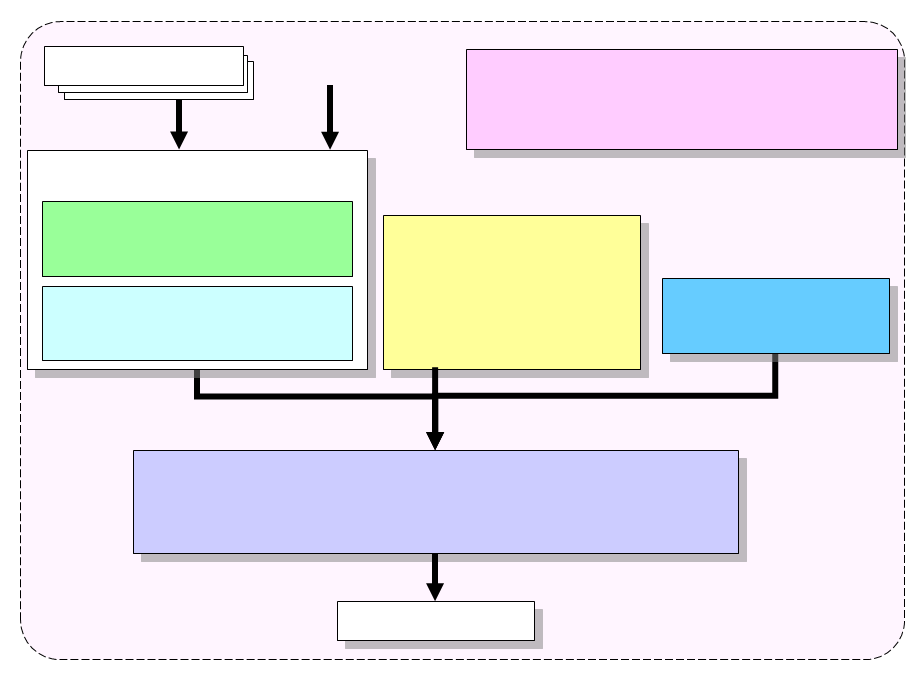
\includegraphics[width=28.5em]{OpenToonzData}}
\put(78,-17){\small 連番画像ファイル}
\put(161,-20){\scriptsize デジタル作画}
\put(237,-20){\small プロジェクトファイル(XML):作品毎}
\put(252,-30){\small ・作業フォルダのパス}
\put(252,-40){\small ・各種設定の既定値}
\put(90,-39){\scriptsize トレース}
\put(93,-59){\small 各セル毎(ラスター)}
\put(77,-75){\small レベルファイル(TLV)}
\put(91,-87){\small ・連番ラスタ画像情報}
\put(77,-107){\small パレットファイル(TPL)}
\put(91,-119){\small ・パレット情報}
\put(205,-81){\footnotesize 各セル毎(ベクター)}
\put(205,-97){\footnotesize ベクターレベルファイル}
\put(205,-107){\footnotesize (PLI)}
\put(205,-117){\footnotesize ・画像+パレット情報}
\put(310,-104){\small 汎用画像ファイル}
\put(310,-116){\small (背景素材等)}
\put(151,-150){\scriptsize タイムシートに配置}
\put(113,-169){\small シーンファイル(TNZ):各カット毎}
\put(127,-180){\footnotesize ・各素材へのパス}
\put(247,-180){\footnotesize ・工フェクト情報}
\put(127,-191){\footnotesize ・素材、タップの幾何変換情報}
\put(247,-191){\footnotesize ・出力設定}
\put(172,-208){\scriptsize レンダリング}
\put(188,-224){\small 出力(画像/動画)}
\end{picture}\\[-0.5em]

\noindent \hskip 1em \begin{tikzpicture}
\bfseries
\draw[fill=fontgreen,fontgreen]  (33.2em,0em) --  (32.2em,-1em) --  (33.2em,-2em) -- (38.3em,-2em) -- (38.3em,0em) -- cycle;
\node at (35.5em,-1em) {\textcolor{white}{データ管理}};
\draw[fill=fontgreen,fontgreen]  (2.6em,-4em) --  (3.6em,-5em) --  (2.6em,-6em) -- (0em,-6em) -- (0em,-4em) -- cycle;
\node at (1.4em,-5em) {\textcolor{white}{仕上}};
\draw[fill=fontgreen,fontgreen]  (3.3em,-7em) --  (4.3em,-8em) --  (3.3em,-9em) -- (0em,-9em) -- (0em,-7em) -- cycle;
\node at (1.8em,-8em) {\textcolor{white}{色指定}};
\draw[fill=fontgreen,fontgreen]  (2.6em,-12.5em) --  (3.6em,-13.5em) --  (2.6em,-14.5em) -- (0em,-14.5em) -- (0em,-12.5em) -- cycle;
\node at (1.4em,-13.5em) {\textcolor{white}{撮影}};
\end{tikzpicture}\\[3em]

\noindent ① Toonz ラスターレベルファイル\\
\normalsize
セルのラスター画像のデータです。1つのファイルの中に1つのセルのフレーム全ての画像データが入って\\
います。拡張子は .tlv です。(セルを英語で Level と言い、OpenToonz 内でもレベルと呼びます。)\\[0.8em]
\large
② パレットファイル\\
\normalsize
セルのパレットの情報が記述されています。拡張子は .tpl です。テキストで書かれているので、メモ帳等の\\
テキストエディタで内容を確認することができます。\\[0.2em]
\uline{★1つのセルにつき、TLV ファイルと同名の TPL ファイルのペアがあります。}\\[0.8em]
\large
③ Toonz ベクターレベルファイル\\
\normalsize
ベクターで描かれたセルのデータです。1つのファイルの中に1つのセルのフレーム全ての画像データと、\\
パレットの情報が両方入っています。拡張子は .pli です。\\[0.8em]
\large
④ シーンファイル\\
\normalsize
各カットの情報がテキストで記述されています。素材となるファイル (Toonz レベルや、背景画像など) の\\
パスや、エフェクトの情報、幾何変換の情報、出力設定などが入っています。拡張子は .tnz です。\\[0.8em]
\large
⑤ プロジェクトファイル\\
\normalsize
作品毎のデータの置き場所 (プロジェクトフォルダ) のパスや、シーン設定の既定値が記述されています。\\
XML の形式で記述されています。\\[2em]
おおまかに言うと、色指定、仕上の工程がそれぞれパレットファイル (TPL)、レベルファイル (TLV) を完\\
成させ、そうして出来た各セルのデータと、背景素材と合成してシーンファイル (TNZ) を完成させるのが、\\
撮影の工程ということになります。

\newpage

\phantomsection
\section*{\uline{\hskip -3em \hskip 3em □ OpenToonz インターフェース\hskip 3.5em}}
\addcontentsline{toc}{section}{□ OpenToonz インターフェース}

\normalsize
\noindent OpenToonz のインターフェースは、機能ごとに様々な「パネル」が用意されています。ユーザはワークスペー\\
ス (Room) 内でそれらのパネルを自由に組み合わせて用いることができます。

\large
\noindent \begin{picture}(0,0)
\put(4,-137){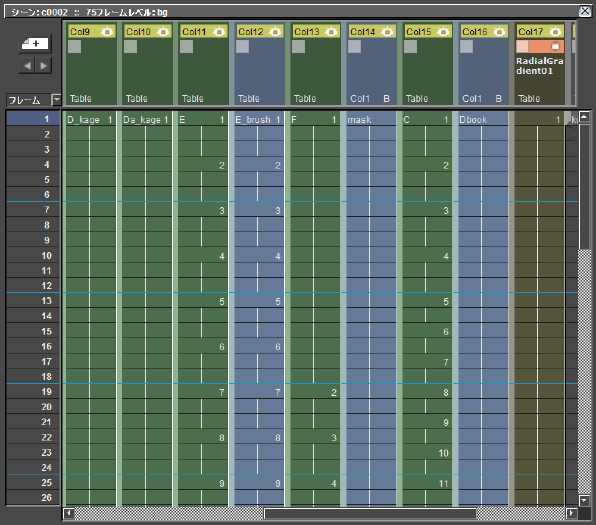
\includegraphics[width=13.8em]{OpenToonzInterfaceXsheet}}
\put(40,-148){\small Xsheet (タイムシート)}
\put(190,-137){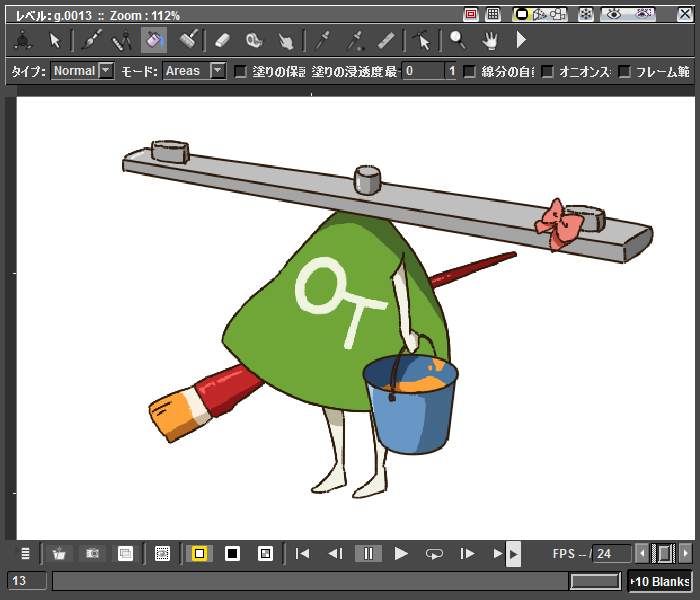
\includegraphics[width=14.15em]{OpenToonzInterfaceComboViewer}}
\put(210,-148){\small Combo Viewer (メインビューア)}
\put(380,-119.5){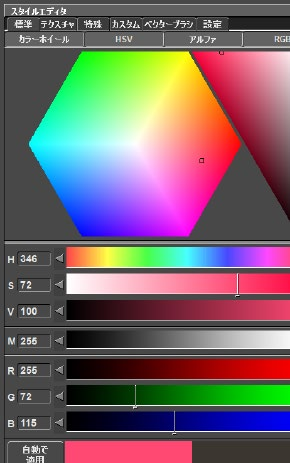
\includegraphics[width=6.7em]{OpenToonzInterfaceStyleEditor}}
\put(393,-128){\small Style Editor}
\put(380,-138){\small (スタイルエディタ)}
\put(4,-292){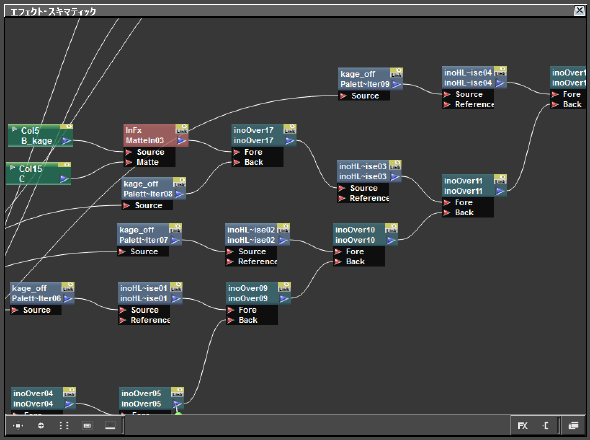
\includegraphics[width=13.8em]{OpenToonzInterfaceSchematic}}
\put(26,-303){\small Schematic (スキマティック)}
\put(184,-248){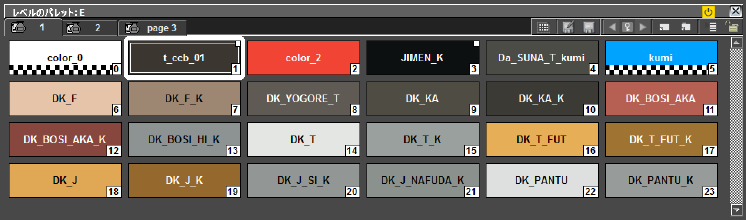
\includegraphics[width=17.2em]{OpenToonzInterfacePalette}}
\put(244,-259){\small Palette (パレット)}
\put(403.6,-335){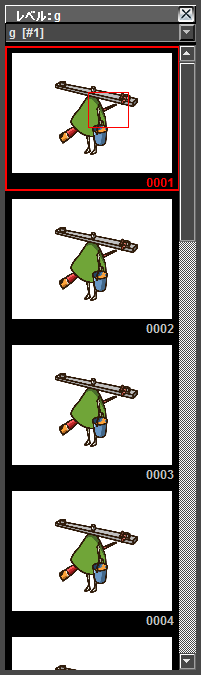
\includegraphics[width=4.7em]{OpenToonzInterfaceLevelStrip}}
\put(255,-290){\small Level Strip (レベルビューア) →}
\end{picture}\\[25.9em]

\normalsize
\noindent ● Xsheet\\
タイムシートのインタフェースです (タイムシートは英語で Exposure Sheet = Xsheet と呼びます)。シー\\
ン内で用いる素材を配置し、各素材の動画番号のタイミングと、簡単な重ね順を決めることができます。\\
● Combo Viewer\\
絵を見ながら行う全ての作業に用います。\\
● Style Editor\\
パレットの色の編集を行うときに用います。カラーホイールと RGB、HSV 値での編集が可能です。\\
● Level Strip\\
編集中のセルの各コマのサムネイルを1列に表示します。\\
● Schematic\\
シーンのエフェクトのかかりかたや、幾何変換の親子関係がツリー構造で表示されるパネルです。\\
● Palette\\
パレットファイルの内容を表示します。\\
他にも、連番画像やムービーを再生するためのパネル「Flipbook(フリップブック)」や、仕上作業のときに\\
色見本を表示して色を拾うためのパネル「Color Model (カラーモデル)」など、様々なパネルがあります。\\
それらはメインウィンドウの各 Room 内にドッキングするか、フローティングウィンドウとして使うことが\\
できます。

\newpage

\phantomsection
\section*{\uline{\hskip -3em \hskip 3em □ Column (列) とレベル\hskip 6.5em}}
\addcontentsline{toc}{section}{□ Column (列) とレベル}

\normalsize
\noindent Xsheet (タイムシート) 上に並べる様々な素材 (セル、背景素材など) のことを、OpenToonz ではまとめて「レ\\
ベル」と呼びます。レベルは Xsheet 上の Column(列) に格納されます。Column のそれぞれの Cell(コマ)に、\\
2つ以上のレベル / 動画番号が入ることはありません。Column は、単に Xsheet 上の配置というだけでなく、\\
OpenToonz のデータ構造上の単位として、重要な意味があります。\\
\large
① Column はレベルの入れ物
\normalsize
\par
- Column の中の1つの Cell は、A) 何も入っていないか、B) 連番ではない\par
\ \ レベルが入っているか、C) 連番画像を持つレベルのあるフレームが入っ\par
\ \ ています。C) の場合、Xsheet にはその動画番号がコマに表示されます。\par
- 撮影作業で OpenToonz のシーンを扱うとき、読み込まれた素材 (レベル)\par
\ \ は全て Xsheet 上に配置しなければ使うことができません。仕上作業でも\par
\ \ 同様で、Xsheet のパネルを表示しないため意識しませんが、LoadLevel で\par
\ \ 読み込まれた Level は Xsheet 上のどれかの Column に配置されています。

\large
\noindent \begin{picture}(0,0)
\put(360,-35){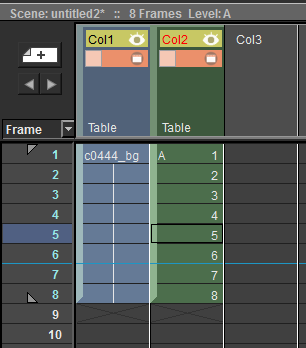
\includegraphics[width=12.1em]{ColumnLevelColumn}}
\end{picture}\\[-15em]

\noindent \hskip 34.2em \begin{tikzpicture}
\draw[->,line width=3pt,red] (0em,-0.8em) to (0em,-2.6em);
\draw[->,line width=3pt,red] (3em,-0.8em) to (3em,-2.6em);
\draw[->,line width=3pt,red] (5.9em,-16.1em) to (5.9em,-14.3em);
\node at (1.5em,0em) {Column};
\node at (4.2em,-16.7em) {空の Column};
\end{tikzpicture}\\[-6.3em]

\noindent ② 移動、リサイズは Column に対して行われる
\normalsize
\par
- 移動、リサイズといった幾何変換情報は、カメラ、テーブル、Pegbar (タッ\par
\ \ プ) またはそれぞれの Column に対して与えることができ、テーブルを親\par
\ \ とした親子関係を持っています。(Stage Schematic)\par
- それぞれの Column の幾何変換情報によって、中に入っている Level の画像が変形されます\\
\\[0.5em]
\large
③ エフェクト合成は Column に対して適用される
\normalsize
\par
- エフェクトも同様に、Column ごとに合成が行われます。Level 素材の入った各 Column ノードをエフェ\par
\ \ クトノードと接続し、Output ノードに繋がる左から右への流れに従ってエフェクト処理が行われます。\par
\ \ (Fx Schematic)\par
- それぞれの Column ノードは、中に入っている Level の画像データを出力します

\large
\noindent \begin{picture}(0,0)
\put(0,-122){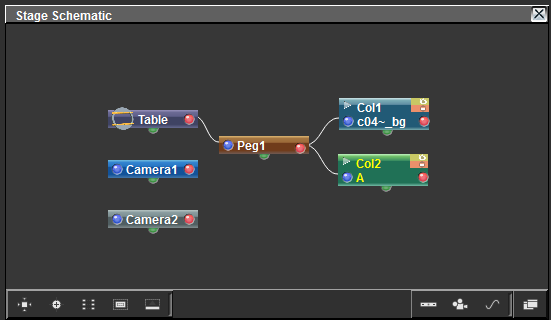
\includegraphics[width=17.8em]{ColumnLevelStageSchematic}}
\put(258,-122){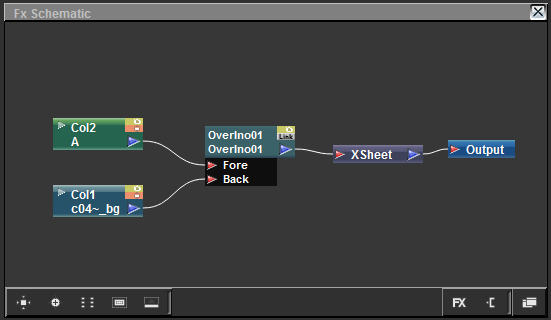
\includegraphics[width=17.8em]{ColumnLevelFxSchematic}}
\end{picture}\\[1.7em]

\noindent \hskip 14em 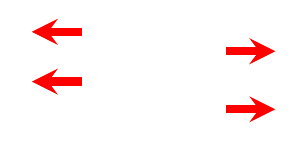
\begin{tikzpicture}
\draw[->,line width=3pt,red] (1.8em,0em) to (0em,0em);
\draw[->,line width=3pt,red] (1.8em,-1.8em) to (0em,-1.8em);
\draw[->,line width=3pt,red] (7em,-0.7em) to (8.8em,-0.7em);
\draw[->,line width=3pt,red] (7em,-2.8em) to (8.8em,-2.8em);
\end{tikzpicture}\\[1.9em]

\small
Stage Schematic (左) と FxSchematic (右)。赤い矢印で示したものが Column ノード (空の Column は表示されない)\\[3em]
\large
※ Xsheet は入れ子構造を取ることができます
\normalsize
\par
\noindent 特殊なケースとして、1 つのレベルの中に、複数の Column のデータを子の Xsheet (= SubXsheet、サブシー\\
ト) としてまとめられる機能があります。複数の Column を選択して、Collapse (サブシートに畳む) コマ\\
ンドを用いると、選択範囲の Column を 1 つの SubXsheet レベルにまとめることができます。

\newpage

\phantomsection
\section*{\uline{\hskip -3em \hskip 3em □シーン編集モードとレベル編集モード}}
\addcontentsline{toc}{section}{□ シーン編集モードとレベル編集モード}

\normalsize
\noindent OpenToonz はアニメーション制作ソフトなので、時系列 (=フレーム) を扱います。OpenToonz には2種\\
類のフレームを選択できるモードがあり、それぞれ、レベルのフレームと、シーンのフレームと呼びます。\\
\\
\large
○レベルのフレーム\\
\normalsize
1 つのレベルを編集しているとき、フレームはそのレベルの持っている動画番号に従います。\\
主に仕上作業のとき、1 つ 1 つのレベルのそれぞれの動画番号の絵に対して作業を行うときは、OpenToonz\\
を\uline{レベル編集モード}に切り替えて下さい。レベル編集モードのときは、Xsheet 上の配置に関係なく、メイ\\
ンビューアには選択中のレベルの現在のフレーム (=動画番号) の絵のみが表示されます。\\
\\
\uline{※ レベル編集モードに切り替えるには}\\
LevelStrip 上に現在のレベルのサムネイルが表示されている状態で、そのサムネイルのひとつを左クリック\\
します。\\[0.5em]
\\
\large
○シーンのフレーム\\
\normalsize
シーンを編集しているとき、フレームは Xsheet の各行番号に従います。\\
主に撮影作業のとき、Xsheet 上に配置された全ての素材を組み合わせて表示しながら作業を行うとき\\
は、OpenToonz を\uline{シーン編集モード}に切り替えてください。シーン編集モードのときは、Xsheet 上で\\
CamStandVisibility (カメラスタンド表示) が ON の Column が全て表示されます。\\
\\
※ レンダリング時およびカメラスタンド表示時の Column の重ね順は、以下の優先順で決まります\par
① Fx Schematic でのレイヤー合成エフェクトの上下関係 (レンダリング時のみ)\par
② Z Depth の値\par
③ SO (Stacking Order、重ね順) の値\par
④ Xsheet 上の並び順 (左が下、右に行くほど上に重なる)\\
\\
\uline{※ シーン編集モードに切り替えるには}\\
Xsheet の左側の、行番号 (=シーンのフレーム) が表示されているエリアを左クリックします。

\large
\noindent \begin{picture}(0,0)
\put(2,-163){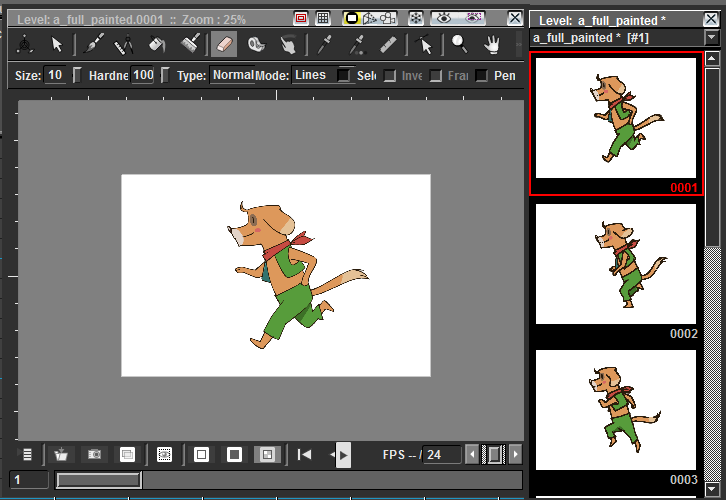
\includegraphics[width=18em]{EditModeLevel}}
\put(240,-163){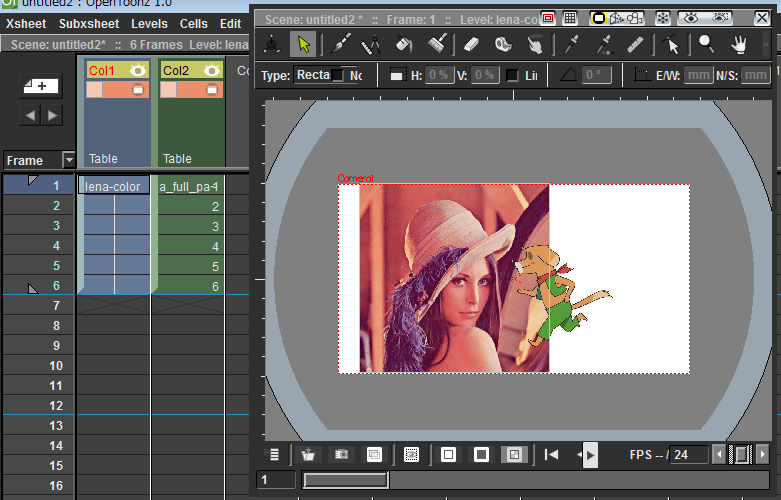
\includegraphics[width=19.35em]{EditModeScene}}
\end{picture}\\[10.5em]

\noindent \hskip 15.3em 
\begin{tikzpicture}
\draw[->,line width=3pt,red] (0em,-1.8em) to (0em,0em);
\draw[->,line width=3pt,red] (5.5em,-1.8em) to (5.5em,0em);
\end{tikzpicture}\\[-2.2em]

\small
\ レベル編集モード (左) とシーン編集モード (右)。それぞれ赤い矢印の部分を左クリックして切り替える。

\newpage

\phantomsection
\section*{\uline{\hskip -3em \hskip 3em □ Room(ワークスペース)\hskip 6.5em}}
\addcontentsline{toc}{section}{□ Room(ワークスペース)}

\normalsize
\noindent OpenToonz は、トレース、色指定、作画&仕上、撮影、バッチ処理、データ管理 の各作業に合わせてパネ\\
ルを組み合わせた Room があらかじめ用意されています。それらは、OpenToonz メインウィンドウの右上\\
の Room タブから切り替えることができます。Room を切り替えると、それに合わせてメニューバーの内容\\
も切り替わります。各 Room のパネルの配置は、ユーザが自由に変更でき、その情報は各ユーザ毎のプロファ\\
イルとして保存され、次回起動時に再現されます。

\large
\noindent \begin{picture}(0,0)
\put(4,-83){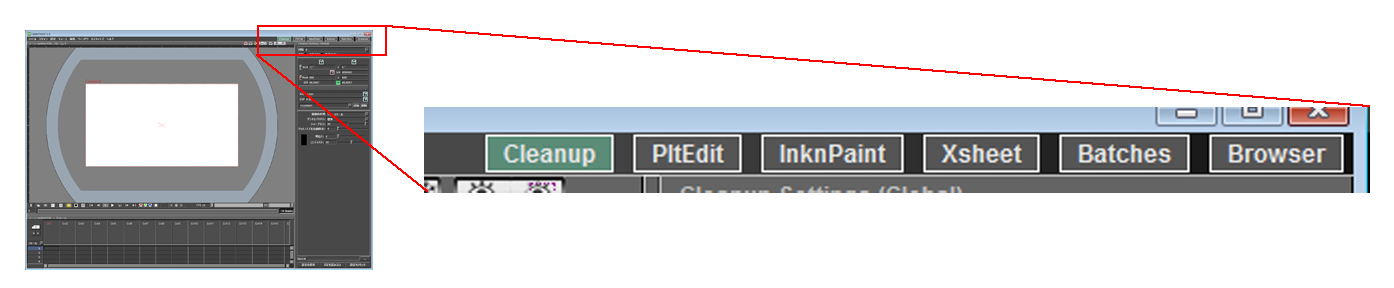
\includegraphics[width=39em]{RoomWorkSpaceTab}}
\put(285,-66){\normalsize Room タブ}
\end{picture}\\[6.4em]

\noindent ● 必要な Room だけ限定して起動するには \normalsize \colorbox{fontyellow}{\color{black}中級}\\
アニメーション制作の各工程を分担して作業する場合、必要な Room だけ限定して起動するようなショート\\
カットを用意しておくと、起動が早くなります。\\
例: "InknPaint" と "Browser" Room のみを開いて起動したい場合\\
① [\$TOONZPROFILES]/layouts/OpenToonz.[ユーザ名] フォルダ内で作業をします。\par
\ (デフォルトでは、OpenToonz Stuff/profiles/layouts/OpenToonz.[ユーザ名])\\
② layouts.txt をコピーし、適当な名前に変更します。(例:shiage\_layout.txt)\\
③ shiage\_layout.txt をワードパッドなどで開くと、下のように Room の設定ファイル名が並んでいますので、\\
対応する Room ("InknPaint" は room3.ini、"Browser" は room6.ini) のみを残して他の行を消し、上書き保\\
存します。\\[-1em]
\par
\ \ \ \ \ \ \ \ room1.ini \ \ \ \ \ \ \ \ \ \ \ \ room3.ini\par
\ \ \ \ \ \ \ \ room2.ini \ \ \ \ \ \ \ \ \ \ \ \ room6.ini\par
\ \ \ \ \ \ \ \ room3.ini\par
\ \ \ \ \ \ \ \ room4.ini\par
\ \ \ \ \ \ \ \ room5.ini\par
\ \ \ \ \ \ \ \ room6.ini

\large
\noindent \begin{picture}(0,0)
\linethickness{0.1em}
\put(42,119){\line(1,0){67}}
\put(109,119){\line(0,-1){105}}
\put(109,14){\line(-1,0){67}}
\put(42,119){\line(0,-1){105}}
\put(153,119){\line(1,0){67}}
\put(221,119){\line(0,-1){105}}
\put(221,14){\line(-1,0){67}}
\put(153,119){\line(0,-1){105}}
\put(228,40){
\includegraphics[width=17em]{RoomWorkSpaceSpeechBubble}}
\put(251,61){\small 必要な Room の設定ファイル名のみを残す}
\end{picture}\\[-8em]

\noindent \hskip 9.7em 
\begin{tikzpicture}
\draw[fill=arrowblue,arrowblue]  (1.6em,0em) --  (2.5em,-0.8em) --  (1.6em,-1.6em) -- (1.6em,-1.0em) -- (0em,-1.0em) -- (0em,-0.6em) -- (1.6em,-0.6em) -- cycle;
\end{tikzpicture}\\[2.5em]

\normalsize
\noindent ④ OpenToonz 実行ファイルのショートカットを作成します\\
⑤ ショートカットを右クリックし、プロパティを開きます\\
⑥ 「リンク先」 に書かれている文字列の末尾に、\par
\ \ -layout shiage\_layout.txt\par
と追加し、OK します。\\
⑦ そのショートカットを用いて OpenToonz を起動すると、\par
指定した Room のみが作られます。

\large
\noindent \begin{picture}(0,0)
\put(273,-57){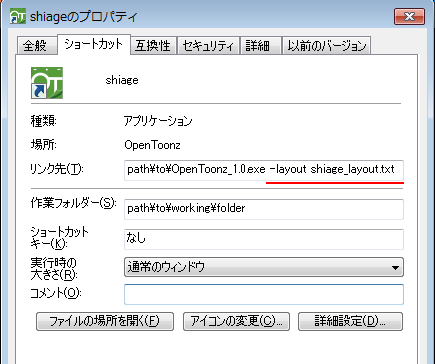
\includegraphics[width=18.7em]{RoomWorkSpaceShiageLayout}}
\put(11,-30){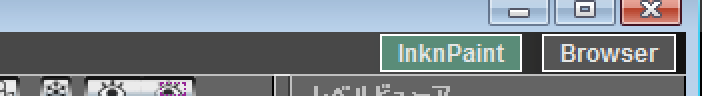
\includegraphics[width=20em]{RoomWorkSpaceInknPaintBrowser}}
\end{picture}

\newpage

\phantomsection
\section*{\uline{\hskip -3em \hskip 3em □プロジェクト毎のデータ管理\hskip 4em}}
\addcontentsline{toc}{section}{□ プロジェクト毎のデータ管理}

\normalsize
\noindent OpenToonz は、各作品を「プロジェクト」と呼び、プロジェクト毎に各工程の素材を置くための作業フォ\\
ルダ(プロジェクトフォルダ)のパスや、プロジェクト内で新規作成されるシーンの設定の既定値などをプ\\
ロジェクト設定として保存することができます。\\
\\
\large
● sandbox プロジェクト\\
\normalsize
初めてOpenToonzを起動したとき、現在のプロジェクトはsandboxという、デフォ\\
ルトのプロジェクトになっています。FileBrowserパネル内左側のフォルダツリー\\
を見ると、"sandbox"というノード名の左側の丸が、赤くなっています。これが、\\
現在 sandbox プロジェクトが選択されているという印です。

\large
\noindent \begin{picture}(0,0)
\put(365,-35){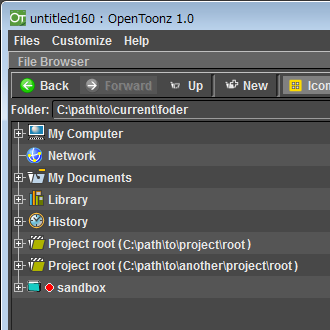
\includegraphics[width=13.2em]{ProjectDataManagementSandboxProject}}
\end{picture}\\

\noindent ● プロジェクトを作成するには\\
\normalsize
① Browser ワークスペース内のメニューバーから、File > New Project を選択し、以下の入力ボックスに、\\
各プロジェクトフォルダへのパスを指定します。\\
\par
\hskip 21em ←プロジェクト設定ファイルの格納先を選択します\\
\par
\hskip 21em ←プロジェクト名\\[-1em]
\par
\small
\hskip 26em プロジェクトフォルダへのパスを入力します。\par
\hskip 26em 以下のようにファイルを入れると想定されています。\par
\hskip 26em +inputs: スキャン画像 (TIF など)\par
\hskip 26em +drawings: Toonz レベル素材 (TLV + PLT と PLI)\par
\hskip 26em +scenes: シーンファイル (TNZ)\par
\hskip 26em +extras: 背景画像ファイル、音声ファイルなど\par
\hskip 26em +outputs: レンダリングされた画像\par
\hskip 26em +palettes: 作品の色見本 (PLT)。Studio Palette パネル内\par
\hskip 26em で Project Palette として参照されます。\par
\hskip 26em +scripts: スクリプトファイル

\large
\noindent \begin{picture}(0,0)
\put(-2,20){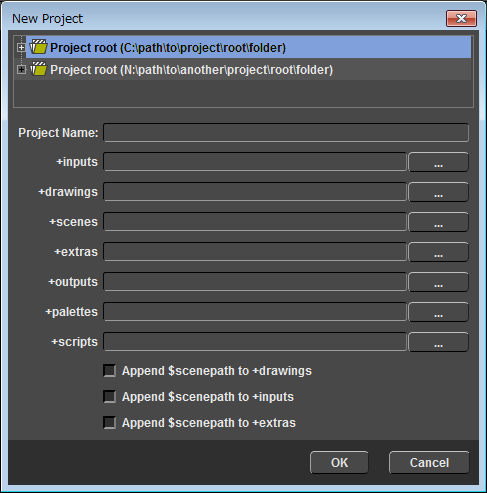
\includegraphics[width=18.2em]{ProjectDataManagementCreateProject}}
\linethickness{0.1em}
\put(223,170){\line(1,0){9}}
\put(232,161){\line(1,0){9}}
\put(232,170){\line(0,-1){92}}
\put(223,78){\line(1,0){9}}
\end{picture}\\[-2.5em]

\normalsize
\noindent ※ \$scenepath という文字列をパス内に用いると、ファイル保存時の現在のシーン名が代入されます。\\
\\
② OK を押すと、プロジェクトが作成され、現在のプロジェクトになります。\\
FileBrowserパネル内左側のフォルダツリーに、新しいプロジェクトノードが追加\\
され、赤い印が移動しています。\\
\\
\large
● プロジェクトを切り替えるには\\
\normalsize
プロジェクトノード名左側の丸をクリックすると、現在のプロジェクトが切り替\\
わり、丸が赤くマークされます。

\large
\noindent \begin{picture}(0,0)
\put(365,-25){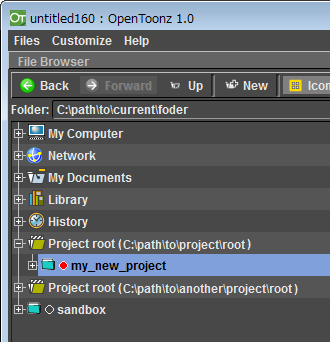
\includegraphics[width=13.2em]{ProjectDataManagementSwitchProject}}
\end{picture}\\

\newpage

\noindent● プロジェクトフォルダを変更するには\\
\normalsize
Browser Room 内で、Files > Project Settings... を実行します。プロジェクトフォルダパスを編集し、ダイア\\
ログを閉じます。\\
\large
● 現在のシーンの設定をプロジェクトの規定値にするには\\
\normalsize
Browser Room 内で、Files > Save Default Settings を実行します。\\
\\[0.5em]
\large
● プロジェクトを作らないで作業を行う\\
\normalsize
プロジェクトに基づくデータ管理は、素材のファイルパスを "+drawings" などのエイリアスに短縮すること\\
で、管理を簡便にすることができ、また、プロジェクトに共通のシーン設定を既定値として持つことができ\\
る、といった利点があります。\\
一方で、仕上の外注作業を行うときなど、様々な作品のデータを少しずつ扱うような使い方をする場合には、\\
作品毎にデータをまとめる利点は少なく、プロジェクトを作る手間が増える分、不便になってしまいます。\\
そのような場合は、プロジェクトを作らず、デフォルトのプロジェクト "sandbox" を選択したまま作業を行っ\\
てください。ユーザの作成したプロジェクトのプロジェクトフォルダおよびそのサブフォルダの外に保存さ\\
れたシーンファイルは、全て sandbox プロジェクトに属していると認識されますので、ユーザはプロジェク\\
トを意識することなく作業を進めることも可能です。\\

\end{document}